\chapter{Teoría de números}

\index{teoría de números}

La \key{teoría de números} es una rama de las matemáticas
que estudia los números enteros.
La teoría de números es un campo fascinante,
porque muchas preguntas que involucran enteros
son muy difíciles de resolver aunque
parezcan sencillas a primera vista.

Como ejemplo, considera la siguiente ecuación:
\[x^3 + y^3 + z^3 = 33\]
Es fácil encontrar tres números reales $x$, $y$ y $z$
que satisfagan la ecuación.
Por ejemplo, podemos elegir
\[
\begin{array}{lcl}
x = 3, \\
y = \sqrt[3]{3}, \\
z = \sqrt[3]{3}.\\
\end{array}
\]
Sin embargo, es un problema abierto en teoría de números
si existen tres
\emph{enteros} $x$, $y$ y $z$
que satisfagan la ecuación \cite{bec07}.

En este capítulo, nos centraremos en los conceptos básicos
y los algoritmos de la teoría de números.
A lo largo del capítulo, supondremos que todos los números
son enteros, si no se indica lo contrario.

\section{Primos y factores}

\index{divisibilidad}
\index{factor}
\index{divisor}

Un número $a$ se llama \key{factor} o \key{divisor} de un número $b$
si $a$ divide a $b$.
Si $a$ es un factor de $b$,
escribimos $a \mid b$, y en caso contrario escribimos $a \nmid b$.
Por ejemplo, los factores de 24 son
1, 2, 3, 4, 6, 8, 12 y 24.

\index{primo}
\index{descomposición en primos}

Un número $n>1$ es \key{primo}
si sus únicos factores positivos son 1 y $n$.
Por ejemplo, 7, 19 y 41 son primos,
pero 35 no es primo, porque $5 \cdot 7 = 35$.
Para cada número $n>1$, existe una única
\key{factorización en primos}
\[ n = p_1^{\alpha_1} p_2^{\alpha_2} \cdots p_k^{\alpha_k},\]
donde $p_1,p_2,\ldots,p_k$ son primos distintos y
$\alpha_1,\alpha_2,\ldots,\alpha_k$ son números positivos.
Por ejemplo, la factorización en primos de 84 es
\[84 = 2^2 \cdot 3^1 \cdot 7^1.\]

El \key{número de factores} de un número $n$ es
\[\tau(n)=\prod_{i=1}^k (\alpha_i+1),\]
porque para cada primo $p_i$, hay
$\alpha_i+1$ formas de elegir cuántas veces
aparece en el factor.
Por ejemplo, el número de factores
de 84 es
$\tau(84)=3 \cdot 2 \cdot 2 = 12$.
Los factores son
1, 2, 3, 4, 6, 7, 12, 14, 21, 28, 42 y 84.

La \key{suma de factores} de $n$ es
\[\sigma(n)=\prod_{i=1}^k (1+p_i+\ldots+p_i^{\alpha_i}) = \prod_{i=1}^k \frac{p_i^{a_i+1}-1}{p_i-1},\]
donde esta última fórmula se basa en la fórmula de la progresión geométrica.
Por ejemplo, la suma de factores de 84 es
\[\sigma(84)=\frac{2^3-1}{2-1} \cdot \frac{3^2-1}{3-1} \cdot \frac{7^2-1}{7-1} = 7 \cdot 4 \cdot 8 = 224.\]

El \key{producto de factores} de $n$ es
\[\mu(n)=n^{\tau(n)/2},\]
porque podemos formar $\tau(n)/2$ pares con los factores,
cada uno con producto $n$.
Por ejemplo, los factores de 84
producen los pares
$1 \cdot 84$, $2 \cdot 42$, $3 \cdot 28$, etc.,
y el producto de los factores es $\mu(84)=84^6=351298031616$.

\index{número perfecto}

Un número $n$ se llama \key{número perfecto} si $n=\sigma(n)-n$,
es decir, $n$ es igual a la suma de sus factores
entre $1$ y $n-1$.
Por ejemplo, 28 es un número perfecto,
porque $28=1+2+4+7+14$.

\subsubsection{Número de primos}

Es fácil demostrar que hay un número infinito
de primos.
Si el número de primos fuera finito,
podríamos construir un conjunto $P=\{p_1,p_2,\ldots,p_n\}$
que contuviera todos los primos.
Por ejemplo, $p_1=2$, $p_2=3$, $p_3=5$, y así sucesivamente.
Sin embargo, usando $P$, podríamos formar un nuevo primo
\[p_1 p_2 \cdots p_n+1\]
que es mayor que todos los elementos de $P$.
Esto es una contradicción, y el número de primos
tiene que ser infinito.

\subsubsection{Densidad de primos}

La densidad de primos significa con qué frecuencia hay primos
entre los números.
Sea $\pi(n)$ el número de primos entre
$1$ y $n$. Por ejemplo, $\pi(10)=4$, porque
hay 4 primos entre $1$ y $10$: 2, 3, 5 y 7.

Es posible demostrar que
\[\pi(n) \approx \frac{n}{\ln n},\]
lo que significa que los primos son bastante frecuentes.
Por ejemplo, el número de primos entre
$1$ y $10^6$ es $\pi(10^6)=78498$,
y $10^6 / \ln 10^6 \approx 72382$.

\subsubsection{Conjeturas}

Hay muchas \emph{conjeturas} que involucran primos.
La mayoría de la gente cree que las conjeturas son ciertas,
pero nadie ha sido capaz de demostrarlas.
Por ejemplo, las siguientes conjeturas son famosas:

\begin{itemize}
\index{conjetura de Goldbach}
\item \key{Conjetura de Goldbach}:
Cada entero par $n>2$ puede representarse como una
suma $n=a+b$ tal que tanto $a$ como $b$ son primos.
\index{primo gemelo}
\item \key{Conjetura de los primos gemelos}:
Hay un número infinito de pares
de la forma $\{p,p+2\}$,
donde tanto $p$ como $p+2$ son primos.
\index{conjetura de Legendre}
\item \key{Conjetura de Legendre}:
Siempre hay un primo entre los números
$n^2$ y $(n+1)^2$, donde $n$ es cualquier entero positivo.
\end{itemize}

\subsubsection{Algoritmos básicos}

Si un número $n$ no es primo,
puede representarse como un producto $a \cdot b$,
donde $a \le \sqrt n$ o $b \le \sqrt n$,
así que ciertamente tiene un factor entre $2$ y $\lfloor \sqrt n \rfloor$.
Usando esta observación, podemos tanto comprobar
si un número es primo como encontrar la factorización en primos
de un número en tiempo $O(\sqrt n)$.

La siguiente función \texttt{prime} comprueba
si el número dado $n$ es primo.
La función intenta dividir $n$ entre
todos los números entre $2$ y $\lfloor \sqrt n \rfloor$,
y si ninguno de ellos divide a $n$, entonces $n$ es primo.

\begin{lstlisting}
bool prime(int n) {
    if (n < 2) return false;
    for (int x = 2; x*x <= n; x++) {
        if (n%x == 0) return false;
    }
    return true;
}
\end{lstlisting}

\noindent
La siguiente función \texttt{factors}
construye un vector que contiene la factorización
en primos de $n$.
La función divide $n$ entre sus factores primos,
y los añade al vector.
El proceso termina cuando el número restante $n$
no tiene factores entre $2$ y $\lfloor \sqrt n \rfloor$.
Si $n>1$, es primo y el último factor.

\begin{lstlisting}
vector<int> factors(int n) {
    vector<int> f;
    for (int x = 2; x*x <= n; x++) {
        while (n%x == 0) {
            f.push_back(x);
            n /= x;
        }
    }
    if (n > 1) f.push_back(n);
    return f;
}
\end{lstlisting}

Nótese que cada factor primo aparece en el vector
tantas veces como divide al número.
Por ejemplo, $24=2^3 \cdot 3$,
así que el resultado de la función es $[2,2,2,3]$.

\subsubsection{Criba de Eratóstenes}

\index{criba de Eratóstenes}

La \key{criba de Eratóstenes}
%\footnote{Eratosthenes (c. 276 BC -- c. 194 BC) was a Greek mathematician.}
es un algoritmo
de preprocesamiento que construye un arreglo con el que
podemos comprobar eficientemente si un número dado entre $2 \ldots n$
es primo y, si no lo es, encontrar un factor primo del número.

El algoritmo construye un arreglo $\texttt{sieve}$
cuyas posiciones $2,3,\ldots,n$ se utilizan.
El valor $\texttt{sieve}[k]=0$ significa
que $k$ es primo,
y el valor $\texttt{sieve}[k] \neq 0$
significa que $k$ no es primo y uno
de sus factores primos es $\texttt{sieve}[k]$.

El algoritmo itera a través de los números
$2 \ldots n$ uno por uno.
Siempre que se encuentra un nuevo primo $x$,
el algoritmo registra que los múltiplos
de $x$ ($2x,3x,4x,\ldots$) no son primos,
porque el número $x$ los divide.

Por ejemplo, si $n=20$, el arreglo es el siguiente:

\begin{center}
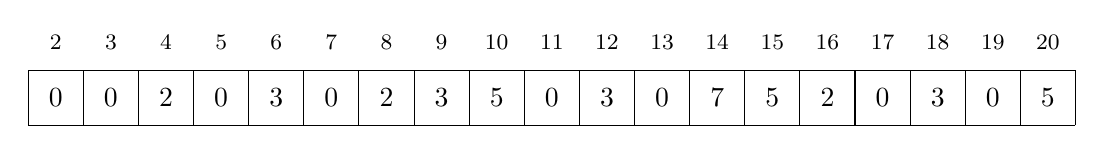
\begin{tikzpicture}[scale=0.7]
\draw (0,0) grid (19,1);

\node at (0.5,0.5) {$0$};
\node at (1.5,0.5) {$0$};
\node at (2.5,0.5) {$2$};
\node at (3.5,0.5) {$0$};
\node at (4.5,0.5) {$3$};
\node at (5.5,0.5) {$0$};
\node at (6.5,0.5) {$2$};
\node at (7.5,0.5) {$3$};
\node at (8.5,0.5) {$5$};
\node at (9.5,0.5) {$0$};
\node at (10.5,0.5) {$3$};
\node at (11.5,0.5) {$0$};
\node at (12.5,0.5) {$7$};
\node at (13.5,0.5) {$5$};
\node at (14.5,0.5) {$2$};
\node at (15.5,0.5) {$0$};
\node at (16.5,0.5) {$3$};
\node at (17.5,0.5) {$0$};
\node at (18.5,0.5) {$5$};

\footnotesize

\node at (0.5,1.5) {$2$};
\node at (1.5,1.5) {$3$};
\node at (2.5,1.5) {$4$};
\node at (3.5,1.5) {$5$};
\node at (4.5,1.5) {$6$};
\node at (5.5,1.5) {$7$};
\node at (6.5,1.5) {$8$};
\node at (7.5,1.5) {$9$};
\node at (8.5,1.5) {$10$};
\node at (9.5,1.5) {$11$};
\node at (10.5,1.5) {$12$};
\node at (11.5,1.5) {$13$};
\node at (12.5,1.5) {$14$};
\node at (13.5,1.5) {$15$};
\node at (14.5,1.5) {$16$};
\node at (15.5,1.5) {$17$};
\node at (16.5,1.5) {$18$};
\node at (17.5,1.5) {$19$};
\node at (18.5,1.5) {$20$};

\end{tikzpicture}
\end{center}

El siguiente código implementa la criba de
Eratóstenes.
El código supone que cada elemento de
\texttt{sieve} es inicialmente cero.

\begin{lstlisting}
for (int x = 2; x <= n; x++) {
    if (sieve[x]) continue;
    for (int u = 2*x; u <= n; u += x) {
        sieve[u] = x;
    }
}
\end{lstlisting}

El bucle interior del algoritmo se ejecuta
$n/x$ veces para cada valor de $x$.
Así, una cota superior para el tiempo de ejecución
del algoritmo es la suma armónica
\[\sum_{x=2}^n n/x = n/2 + n/3 + n/4 + \cdots + n/n = O(n \log n).\]

\index{suma armónica}

De hecho, el algoritmo es más eficiente,
porque el bucle interior solo se ejecutará si
el número $x$ es primo.
Se puede demostrar que el tiempo de ejecución del
algoritmo es solo $O(n \log \log n)$,
una complejidad muy cercana a $O(n)$.

\subsubsection{Algoritmo de Euclides}

\index{máximo común divisor}
\index{mínimo común múltiplo}
\index{algoritmo de Euclides}

El \key{máximo común divisor} de
los números $a$ y $b$, $\gcd(a,b)$,
es el mayor número que divide tanto a $a$ como a $b$,
y el \key{mínimo común múltiplo} de
$a$ y $b$, $\textrm{lcm}(a,b)$,
es el menor número que es divisible por
tanto $a$ como $b$.
Por ejemplo,
$\gcd(24,36)=12$ y
$\textrm{lcm}(24,36)=72$.

El máximo común divisor y el mínimo común múltiplo
están relacionados de la siguiente manera:
\[\textrm{lcm}(a,b)=\frac{ab}{\textrm{gcd}(a,b)}\]

El \key{algoritmo de Euclides}\footnote{Euclides fue un matemático griego que
vivió alrededor del año 300 a. C. Este es quizás el primer algoritmo conocido de la historia.} proporciona una forma eficiente
de encontrar el máximo común divisor de dos números.
El algoritmo se basa en la siguiente fórmula:
\begin{equation*}
    \textrm{gcd}(a,b) = \begin{cases}
               a        & b = 0\\
               \textrm{gcd}(b,a \bmod b) & b \neq 0\\
           \end{cases}
\end{equation*}

Por ejemplo,
\[\textrm{gcd}(24,36) = \textrm{gcd}(36,24)
= \textrm{gcd}(24,12) = \textrm{gcd}(12,0)=12.\]

El algoritmo se puede implementar de la siguiente manera:
\begin{lstlisting}
int gcd(int a, int b) {
    if (b == 0) return a;
    return gcd(b, a%b);
}
\end{lstlisting}

Se puede demostrar que el algoritmo de Euclides funciona
en tiempo $O(\log n)$, donde $n=\min(a,b)$.
El peor caso para el algoritmo es
el caso en que $a$ y $b$ son números de Fibonacci consecutivos.
Por ejemplo,
\[\textrm{gcd}(13,8)=\textrm{gcd}(8,5)
=\textrm{gcd}(5,3)=\textrm{gcd}(3,2)=\textrm{gcd}(2,1)=\textrm{gcd}(1,0)=1.\]

\subsubsection{Función totiente de Euler}

\index{coprimo}
\index{función totiente de Euler}

Los números $a$ y $b$ son \key{coprimos}
si $\textrm{gcd}(a,b)=1$.
La \key{función totiente de Euler} $\varphi(n)$
%\footnote{Euler presented this function in 1763.}
da el número de números coprimos con $n$
entre $1$ y $n$.
Por ejemplo, $\varphi(12)=4$,
porque 1, 5, 7 y 11
son coprimos con 12.

El valor de $\varphi(n)$ se puede calcular
a partir de la factorización en primos de $n$
usando la fórmula
\[ \varphi(n) = \prod_{i=1}^k p_i^{\alpha_i-1}(p_i-1). \]
Por ejemplo, $\varphi(12)=2^1 \cdot (2-1) \cdot 3^0 \cdot (3-1)=4$.
Nótese que $\varphi(n)=n-1$ si $n$ es primo.

\section{Aritmética modular}

\index{aritmética modular}

En la \key{aritmética modular},
el conjunto de números está limitado de modo
que solo se usan los números $0,1,2,\ldots,m-1$,
donde $m$ es una constante.
Cada número $x$ está
representado por el número $x \bmod m$:
el resto después de dividir $x$ entre $m$.
Por ejemplo, si $m=17$, entonces $75$
está representado por $75 \bmod 17 = 7$.

A menudo podemos tomar los restos antes de realizar
los cálculos.
En particular, se cumplen las siguientes fórmulas:
\[
\begin{array}{rcl}
(x+y) \bmod m & = & (x \bmod m + y \bmod m) \bmod m \\
(x-y) \bmod m & = & (x \bmod m - y \bmod m) \bmod m \\
(x \cdot y) \bmod m & = & (x \bmod m \cdot y \bmod m) \bmod m \\
x^n \bmod m & = & (x \bmod m)^n \bmod m \\
\end{array}
\]

\subsubsection{Exponenciación modular}

A menudo hay necesidad de calcular eficientemente
el valor de $x^n \bmod m$.
Esto se puede hacer en tiempo $O(\log n)$
usando la siguiente recursión:
\begin{equation*}
    x^n = \begin{cases}
               1        & n = 0\\
               x^{n/2} \cdot x^{n/2} & \text{$n$ es par}\\
               x^{n-1} \cdot x & \text{$n$ es impar}
           \end{cases}
\end{equation*}

Es importante que en el caso de un $n$ par,
el valor de $x^{n/2}$ se calcule solo una vez.
Esto garantiza que la complejidad temporal del
algoritmo sea $O(\log n)$, porque $n$ siempre se divide entre dos
cuando es par.

La siguiente función calcula el valor de
$x^n \bmod m$:

\begin{lstlisting}
int modpow(int x, int n, int m) {
    if (n == 0) return 1%m;
    long long u = modpow(x,n/2,m);
    u = (u*u)%m;
    if (n%2 == 1) u = (u*x)%m;
    return u;
}
\end{lstlisting}

\subsubsection{Teorema de Fermat y teorema de Euler}

\index{teorema de Fermat}
\index{teorema de Euler}

El \key{teorema de Fermat}
%\footnote{Fermat discovered this theorem in 1640.}
establece que
\[x^{m-1} \bmod m = 1\]
cuando $m$ es primo y $x$ y $m$ son coprimos.
Esto también da
\[x^k \bmod m = x^{k \bmod (m-1)} \bmod m.\]
Más generalmente, el \key{teorema de Euler}
%\footnote{Euler published this theorem in 1763.}
establece que
\[x^{\varphi(m)} \bmod m = 1\]
cuando $x$ y $m$ son coprimos.
El teorema de Fermat se deriva del teorema de Euler,
porque si $m$ es primo, entonces $\varphi(m)=m-1$.

\subsubsection{Inverso modular}

\index{inverso modular}

El inverso de $x$ módulo $m$
es un número $x^{-1}$ tal que
\[ x x^{-1} \bmod m = 1. \]
Por ejemplo, si $x=6$ y $m=17$,
entonces $x^{-1}=3$, porque $6\cdot3 \bmod 17=1$.

Usando inversos modulares, podemos dividir números
módulo $m$, porque la división por $x$
corresponde a la multiplicación por $x^{-1}$.
Por ejemplo, para evaluar el valor de $36/6 \bmod 17$,
podemos usar la fórmula $2 \cdot 3 \bmod 17$,
porque $36 \bmod 17 = 2$ y $6^{-1} \bmod 17 = 3$.

Sin embargo, un inverso modular no siempre existe.
Por ejemplo, si $x=2$ y $m=4$, la ecuación
\[ x x^{-1} \bmod m = 1 \]
no se puede resolver, porque todos los múltiplos de 2
son pares y el resto nunca puede ser 1 cuando $m=4$.
Resulta que el valor de $x^{-1} \bmod m$
se puede calcular exactamente cuando $x$ y $m$ son coprimos.

Si existe un inverso modular, se puede
calcular usando la fórmula
\[
x^{-1} = x^{\varphi(m)-1}.
\]
Si $m$ es primo, la fórmula se convierte en
\[
x^{-1} = x^{m-2}.
\]
Por ejemplo,
\[6^{-1} \bmod 17 =6^{17-2} \bmod 17 = 3.\]

Esta fórmula nos permite calcular eficientemente
los inversos modulares usando el algoritmo de exponenciación modular.
La fórmula se puede derivar usando el teorema de Euler.
Primero, el inverso modular debe satisfacer la siguiente ecuación:
\[
x x^{-1} \bmod m = 1.
\]
Por otro lado, según el teorema de Euler,
\[
x^{\varphi(m)} \bmod m =  xx^{\varphi(m)-1} \bmod m = 1,
\]
así que los números $x^{-1}$ y $x^{\varphi(m)-1}$ son iguales.

\subsubsection{Aritmética de computadora}

En programación, los enteros sin signo se representan módulo $2^k$,
donde $k$ es el número de bits del tipo de dato.
Una consecuencia habitual de esto es que un número se envuelve
si se vuelve demasiado grande.

Por ejemplo, en C++, los números de tipo \texttt{unsigned int}
se representan módulo $2^{32}$.
El siguiente código declara una variable
\texttt{unsigned int} cuyo valor es $123456789$.
Después de esto, el valor se multiplicará por sí mismo,
y el resultado es
$123456789^2 \bmod 2^{32} = 2537071545$.

\begin{lstlisting}
unsigned int x = 123456789;
cout << x*x << "\n"; // 2537071545
\end{lstlisting}

\section{Resolución de ecuaciones}

\subsubsection*{Ecuaciones diofánticas}

\index{ecuación diofántica}

Una \key{ecuación diofántica}
%\footnote{Diophantus of Alexandria was a Greek mathematician who lived in the 3th century.}
es una ecuación de la forma
\[ ax + by = c, \]
donde $a$, $b$ y $c$ son constantes
y hay que encontrar los valores de $x$ e $y$.
Cada número de la ecuación tiene que ser un entero.
Por ejemplo, una solución para la ecuación
$5x+2y=11$ es $x=3$ e $y=-2$.

\index{algoritmo extendido de Euclides}

Podemos resolver eficientemente una ecuación diofántica
usando el algoritmo de Euclides.
Resulta que podemos extender el algoritmo de Euclides
de modo que encuentre números $x$ e $y$
que satisfagan la siguiente ecuación:
\[
ax + by = \textrm{gcd}(a,b)
\]

Una ecuación diofántica se puede resolver si
$c$ es divisible por
$\textrm{gcd}(a,b)$,
y en caso contrario no se puede resolver.

Como ejemplo, encontremos números $x$ e $y$
que satisfagan la siguiente ecuación:
\[
39x + 15y = 12
\]
La ecuación se puede resolver, porque
$\textrm{gcd}(39,15)=3$ y $3 \mid 12$.
Cuando el algoritmo de Euclides calcula el
máximo común divisor de 39 y 15,
produce la siguiente secuencia de llamadas a función:
\[
\textrm{gcd}(39,15) = \textrm{gcd}(15,9)
= \textrm{gcd}(9,6) = \textrm{gcd}(6,3)
= \textrm{gcd}(3,0) = 3 \]
Esto corresponde a las siguientes ecuaciones:
\[
\begin{array}{lcl}
39 - 2 \cdot 15 & = & 9 \\
15 - 1 \cdot 9 & = & 6 \\
9 - 1 \cdot 6 & = & 3 \\
\end{array}
\]
Usando estas ecuaciones, podemos derivar
\[
39 \cdot 2 + 15 \cdot (-5) = 3
\]
y multiplicando esto por 4, el resultado es
\[
39 \cdot 8 + 15 \cdot (-20) = 12,
\]
así que una solución a la ecuación es
$x=8$ e $y=-20$.

Una solución a una ecuación diofántica no es única,
porque podemos formar un número infinito de soluciones
si conocemos una solución.
Si un par $(x,y)$ es una solución, entonces también todos los pares
\[(x+\frac{kb}{\textrm{gcd}(a,b)},y-\frac{ka}{\textrm{gcd}(a,b)})\]
son soluciones, donde $k$ es cualquier entero.

\subsubsection{Teorema chino del resto}

\index{teorema chino del resto}

El \key{teorema chino del resto} resuelve
un grupo de ecuaciones de la forma
\[
\begin{array}{lcl}
x & = & a_1 \bmod m_1 \\
x & = & a_2 \bmod m_2 \\
\cdots \\
x & = & a_n \bmod m_n \\
\end{array}
\]
donde todos los pares de $m_1,m_2,\ldots,m_n$ son coprimos.

Sea $x^{-1}_m$ el inverso de $x$ módulo $m$, y
\[ X_k = \frac{m_1 m_2 \cdots m_n}{m_k}.\]
Usando esta notación, una solución a las ecuaciones es
\[x = a_1 X_1 {X_1}^{-1}_{m_1} + a_2 X_2 {X_2}^{-1}_{m_2} + \cdots + a_n X_n {X_n}^{-1}_{m_n}.\]
En esta solución, para cada $k=1,2,\ldots,n$,
\[a_k X_k {X_k}^{-1}_{m_k} \bmod m_k = a_k,\]
porque
\[X_k {X_k}^{-1}_{m_k} \bmod m_k = 1.\]
Dado que todos los demás términos de la suma son divisibles por $m_k$,
no tienen efecto en el resto,
y $x \bmod m_k = a_k$.

Por ejemplo, una solución para
\[
\begin{array}{lcl}
x & = & 3 \bmod 5 \\
x & = & 4 \bmod 7 \\
x & = & 2 \bmod 3 \\
\end{array}
\]
es
\[ 3 \cdot 21 \cdot 1 + 4 \cdot 15 \cdot 1 + 2 \cdot 35 \cdot 2 = 263.\]

Una vez que hemos encontrado una solución $x$,
podemos crear un número infinito de otras soluciones,
porque todos los números de la forma
\[x+m_1 m_2 \cdots m_n\]
son soluciones.

\section{Otros resultados}

\subsubsection{Teorema de Lagrange}

\index{teorema de Lagrange}

El \key{teorema de Lagrange}
%\footnote{J.-L. Lagrange (1736--1813) was an Italian mathematician.}
establece que todo entero positivo
puede representarse como una suma de cuatro cuadrados, es decir,
$a^2+b^2+c^2+d^2$.
Por ejemplo, el número 123 puede representarse
como la suma $8^2+5^2+5^2+3^2$.

\subsubsection{Teorema de Zeckendorf}

\index{teorema de Zeckendorf}
\index{número de Fibonacci}

El \key{teorema de Zeckendorf}
%\footnote{E. Zeckendorf published the theorem in 1972 \cite{zec72}; however, this was not a new result.}
establece que todo
entero positivo tiene una representación única
como una suma de números de Fibonacci tal que
no hay dos números que sean iguales o números
de Fibonacci consecutivos.
Por ejemplo, el número 74 puede representarse
como la suma $55+13+5+1$.

\subsubsection{Ternas pitagóricas}

\index{terna pitagórica}
\index{fórmula de Euclides}

Una \key{terna pitagórica} es una terna $(a,b,c)$
que satisface el teorema de Pitágoras
$a^2+b^2=c^2$, lo que significa que hay un triángulo rectángulo
con longitudes de lado $a$, $b$ y $c$.
Por ejemplo, $(3,4,5)$ es una terna pitagórica.

Si $(a,b,c)$ es una terna pitagórica,
todas las ternas de la forma $(ka,kb,kc)$
son también ternas pitagóricas donde $k>1$.
Una terna pitagórica es \emph{primitiva} si
$a$, $b$ y $c$ son coprimos,
y todas las ternas pitagóricas se pueden construir
a partir de ternas primitivas usando un multiplicador $k$.

La \key{fórmula de Euclides} se puede usar para producir
todas las ternas pitagóricas primitivas.
Cada una de tales ternas es de la forma
\[(n^2-m^2,2nm,n^2+m^2),\]
donde $0<m<n$, $n$ y $m$ son coprimos
y al menos uno de $n$ y $m$ es par.
Por ejemplo, cuando $m=1$ y $n=2$, la fórmula
produce la terna pitagórica más pequeña
\[(2^2-1^2,2\cdot2\cdot1,2^2+1^2)=(3,4,5).\]

\subsubsection{Teorema de Wilson}

\index{teorema de Wilson}

El \key{teorema de Wilson}
%\footnote{J. Wilson (1741--1793) was an English mathematician.}
establece que un número $n$
es primo exactamente cuando
\[(n-1)! \bmod n = n-1.\]
Por ejemplo, el número 11 es primo, porque
\[10! \bmod 11 = 10,\]
y el número 12 no es primo, porque
\[11! \bmod 12 = 0 \neq 11.\]

Por tanto, el teorema de Wilson se puede usar para averiguar
si un número es primo. Sin embargo, en la práctica, el teorema no se puede
aplicar a valores grandes de $n$, porque es difícil
calcular valores de $(n-1)!$ cuando $n$ es grande.

